\documentclass[12pt]{article}
\usepackage{mathtools}
\usepackage{amssymb}
\usepackage{amsthm}
\usepackage{pgfplots}
\usepackage{tikz}
\usetikzlibrary{calc}
\usepackage{polski}
\usepackage[utf8]{inputenc}
\usepackage{geometry}
\usepackage{amsmath}
\usepackage{mnsymbol}
\usepackage{graphicx}
\usepackage{textgreek}
\usepackage{float}
\usepackage{caption}
\begin{document}
\newgeometry{tmargin=2cm,bmargin=2cm,lmargin=2cm,rmargin=2cm}
\tableofcontents \newpage
\section{Cel ćwiczenia}
Celem ćwiczenia było wyznaczenie rozkładu natężenia światła laserowego dla obrazu dyfrakcyjnego pojedynczej szczeliny i układu dwóch szczelin oraz obliczenie szerokości szczeliny.
\section{Wstęp teorytyczny}
1. Dzięki zjawisku emisji wymuszonej wszystkie atomy w laserze emitują światło o identycznych własnościach. Jest ono emitowane w wyniku przejść atomów pomiędzy stanami o wyższej a stanami o niższej energii. Atomy te emitują światło w sposób skorelowany. 
Białe światło, takie jak to wysyłane przez Słońce lub żarówki jest mieszaniną fal świetlnych o różnych długościach. Każdej długości fali odpowiada inna barwa światła, jeśli do naszego oka fale takie docierają oddzielnie. Światło jest falą elektromagnetyczną, której długość zawarta jest w przedziale 380-780 nanometrów. Jest to więc niewielki wycinek z całego widma fal elektromagnetycznych. Ludzkie oko czułe jest tylko na fale elektromagnetyczne z tego właśnie zakresu. \newline
2. Fala świetlna padająca na przeszkodę w postaci pojedynczej, wąskiej szczeliny ulega zjawisku dyfrakcji, w wyniku czego na ekranie pojawia się charakterystyczny
obraz dyfrakcyjny, składający się z jasnego maksimum głównego oraz mniej intensywnych, ułożonych na przemian jasnych \newline i ciemnych prążków pobocznych. \newline
3. Szerokość nieznanej szczeliny w oparciu o uzyskany obraz dyfrakcyjny dla światła monochromatycznego możemy uzyskać korzystając ze wzorów dla minimum dyfrakcyjnych oraz maksimum dyfrakcyjnych podanych poniżej: \newline
{\Large $x_{min}=m\frac{\lambda{L}}{d}\;\;\;=>\;\;\; d=m\frac{\lambda{L}}{x_{min}}$} \newline
{\Large $x_{max}=(m+\frac{1}{2})\frac{\lambda{L}}{d}\;\;\; =>\;\;\; d=(m+\frac{1}{2})\frac{\lambda{L}}{x_{max}}$} \newline
Szerokość możemy przyjąć jako średnią arytmetyczną wyników. \newline
4. Przyjęcie odległości szczelina-ekran przynajmniej $70\;cm$ pozwala na osiągnięcie takiego kąta, dla którego możemy skutecznie przyjąć przybliżenie 
$sin(\theta)\approx\frac{x}{L}$ . \newline
5. Przykładowa wartość pierwszego maksimum dyfrakcyjnego dla szczeliny o szerokości $d=0.1\;mm$, długości fali światła laserowego $\lambda=600\;mm$ oraz odległości szczelina-ekran $90\;cm$ wynosi $x_{max}=8.1\;mm$. \newline
6. Schemat elektryczny układu do pomiaru natężenia światła przedstawiony został w punkcie $3$. \newline
7. Stosunek wartości natężenia światła w pierwszym maksimum bocznym ($m=1$) do natężenia maksimum głównego wynosi: \newline
{\Large $ \frac{I(x_{max})}{I_0}\approx\frac{1}{\pi^2(m+\frac{1}{2})^2}\;\;\;=>\;\;\;
\frac{I(x_{max_1})}{I_0}\approx\frac{1}{\pi^2(1+\frac{1}{2})^2}\approx 0.045  $} \newpage
\section{Układ pomiarowy}
Układ pomiarowy składa się z części optycznej oraz układu elektrycznego. \newline
Układ optyczny (Rys. 1) składa się z: \newline
1. Laseru emitującego światło czerwone o długości fali $\lambda=650\;nm$ \newline
2. Przesłony metalowej zawierającej szczelinę podwójną, szczelinę pojedynczą i układ 4 szczelin \newline
3. Ekranu zaopatrzonego w fotodiodę oraz układu jej przesuwu w kierunku poziomym i pionowym \newline
\begin{figure}[H]
\centering
\includegraphics[width=11cm]{1}
\caption*{\textbf{Rys. 1}: Układ optyczny}
\end{figure} 
\noindent Układ elektryczny (Rys. 2) składa się z: \newline
4. Fotodiody \newline
5. Woltomierza cyfrowego o pojedynczym zakresie pomiarowym $400\;mV$ \newline
6. Baterii zasilającej  $2\times1.5\;V$ \newline
7. Opornika regulowanego dekadowego $10\times100\;\Omega$ \newline
8. Dodatkowych oporników $1\;k\Omega$ i $2\;k\Omega$ 
\begin{figure}[H]
\centering
\includegraphics[width=11cm]{2}
\caption*{\textbf{Rys. 2}: Układ elektryczny }
\end{figure} \newpage
\section{Przebieg ćwiczenia}
Po zapoznaniu się z układem eksperymentalnym i podłączeniu układu zasilania detektorem światła przy asyście prowadzącego włączyliśmy zasilanie lasera i układu detekcyjnego. Wyregulowaliśmy położenie pojedynczej szczeliny stałej, tak aby uzyskać jak największą jasność obrazu dyfrakcyjnego. Po ustawieniu wartości oporu $R$ wykonaliśmy szereg pomiarów natężeń światła $I$ w funkcji położenia $x$ w zakresie obejmującym maksimum główne oraz dwa prążki poboczne po obu stronach maksimum głównego (przesuwaliśmy detektor co $0,2mm$.) Te same czynności powtórzyliśmy dla szczeliny podwójnej. Następnie wyłączyliśmy laser i zasilanie fotodiody w celu zmierzenia odległości $L$ od szczeliny do ekranu oraz zapisaliśmy długość fali światła lasera. Przyjęliśmy niepewność pomiaru odległości jako długość działki elementarnej $u(L)=0.1\;mm$.
\newpage
\section{Wyniki pomiarów}
\begin{center}
{\Large \;\;\;\;\;\;\;\;\;\;\;\;\;\;\;\;\;\;\;\;Pojedyncza szczelina}  \newline
Odległość szczelina-fotodioda: $755\;mm$
\end{center}
\begin{figure}[H]
\centering
\includegraphics[width=6.8cm]{Tab1}
\caption*{\textbf{Tab. 1}: Wyniki pomiarów dla pojedynczej szczeliny }
\end{figure} 
\begin{center}
{\Large \;\;\;\;\;\;\;\;\;\;\;\;\;\;\;\;\;\;\;\;Podwójna szczelina}  \newline
Odległość szczelina-fotodioda: $755\;mm$
\end{center}
\begin{figure}[H]
\centering
\includegraphics[width=11cm]{Tab2}
\caption*{\textbf{Tab. 2}: Wyniki pomiarów dla podwójnej szczeliny }
\end{figure} 
\section{Opracowanie wyników pomiarów dla pojedynczej szczeliny}
\subsection{Wykres zależności natężenia światła $I$ od położenia detektora $x$}
\begin{center}
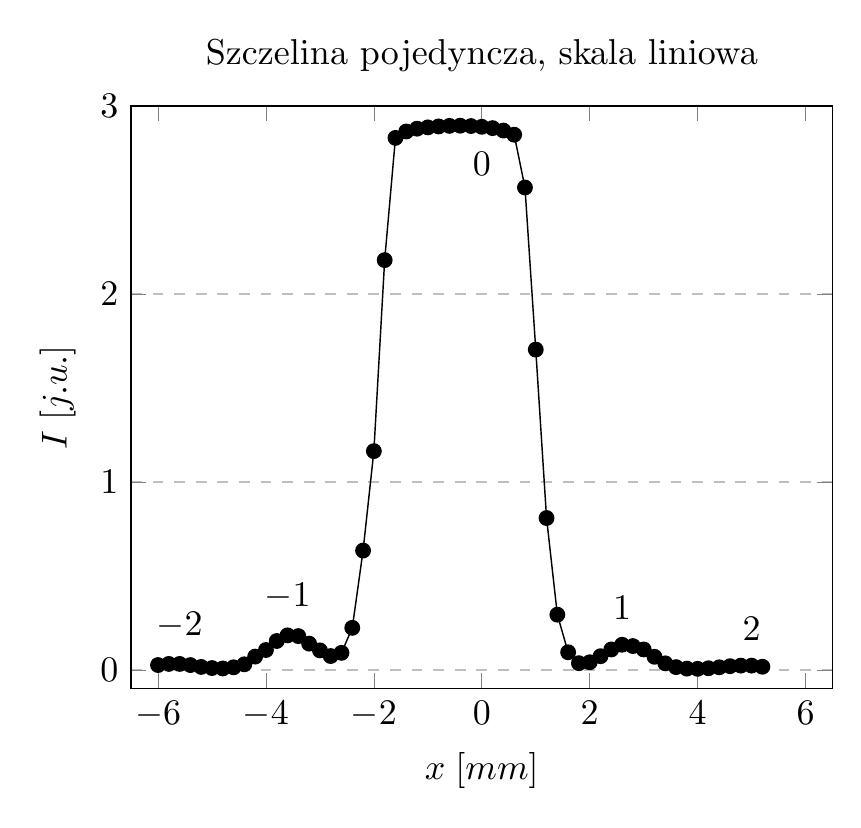
\begin{tikzpicture}[scale=1.3]
\begin{axis}[
title={Szczelina pojedyncza, skala liniowa},
xlabel={$x\;[mm]$},
ylabel={$I\;[j.u.]$},
xmin=-6.5,xmax=6.5,
ymin=-0.1,ymax=3,
legend pos=north west,
ymajorgrids=true,grid style=dashed
]

\addplot[color=black, mark=*]
coordinates {
(-6,0.026)
(-5.8,0.032)
(-5.6,0.032)
(-5.4,0.026)
(-5.2,0.016)
(-5,0.010)
(-4.8,0.008)
(-4.6,0.014)
(-4.4,0.030)
(-4.2,0.071)
(-4,0.106)
(-3.8,0.154)
(-3.6,0.184)
(-3.4,0.180)
(-3.2,0.140)
(-3,0.104)
(-2.8,0.074)
(-2.6,0.091)
(-2.4,0.224)
(-2.2,0.635)
(-2,1.164)
(-1.8,2.180)
(-1.6,2.830)
(-1.4,2.864)
(-1.2,2.879)
(-1,2.886)
(-0.8,2.891)
(-0.6,2.894)
(-0.4,2.895)
(-0.2,2.893)
(0,2.889)
(0.2,2.882)
(0.4,2.869)
(0.6,2.847)
(0.8,2.566)
(1,1.704)
(1.2,0.808)
(1.4,0.294)
(1.6,0.094)
(1.8,0.036)
(2,0.041)
(2.2,0.073)
(2.4,0.109)
(2.6,0.134)
(2.8,0.127)
(3,0.109)
(3.2,0.070)
(3.4,0.035)
(3.6,0.015)
(3.8,0.007)
(4,0.006)
(4.2,0.009)
(4.4,0.014)
(4.6,0.020)
(4.8,0.023)
(5,0.023)
(5.2,0.017)
};
\node[label={270:{$0$}}] at (axis cs: 0,2.888) {};
\node[label={90:{$1$}}] at (axis cs: 2.6,0.131) {};
\node[label={90:{$2$}}] at (axis cs: 5,0.023) {};
\node[label={90:{$-1$}}] at (axis cs: -3.6,0.184) {};
\node[label={90:{$-2$}}] at (axis cs: -5.6,0.031) {};
\end{axis}
\end{tikzpicture}
\end{center}
\begin{center}
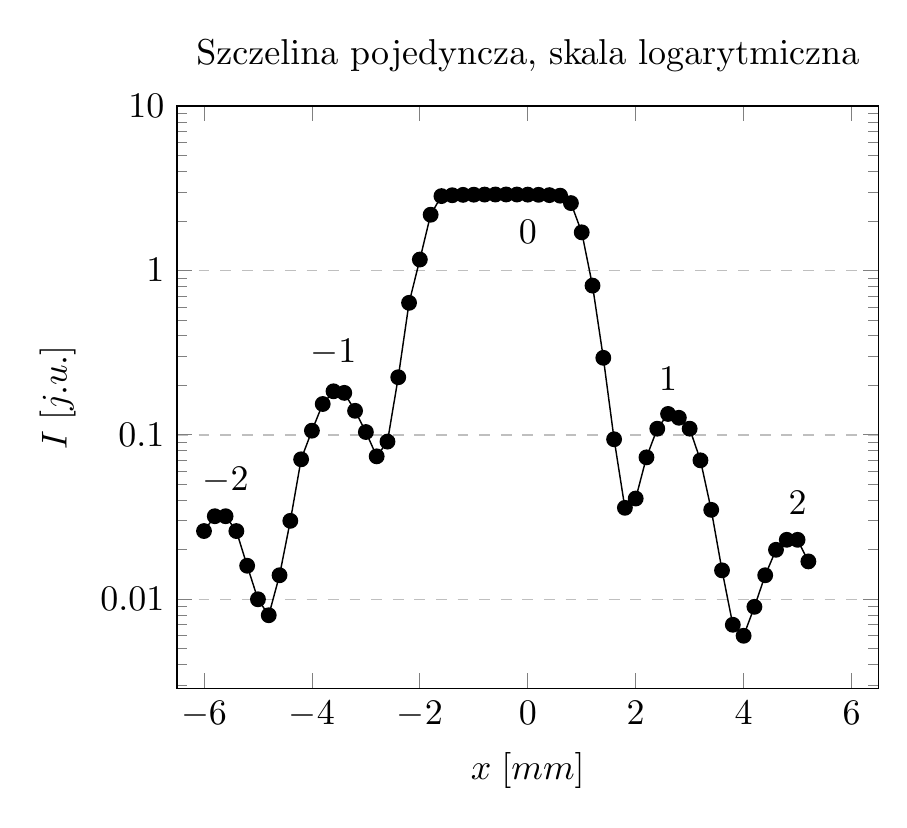
\begin{tikzpicture}[scale=1.3]
\begin{axis}[
title={Szczelina pojedyncza, skala logarytmiczna},
xlabel={$x\;[mm]$},
ylabel={$I\;[j.u.]$},
xmin=-6.5,xmax=6.5,
ymin=-0.1,ymax=10,
legend pos=north west,
ymajorgrids=true,grid style=dashed,
ymode=log,
log ticks with fixed point,
scaled y ticks=real:1e3
]

\addplot[color=black, mark=*]
coordinates {
(-6,0.026)
(-5.8,0.032)
(-5.6,0.032)
(-5.4,0.026)
(-5.2,0.016)
(-5,0.010)
(-4.8,0.008)
(-4.6,0.014)
(-4.4,0.030)
(-4.2,0.071)
(-4,0.106)
(-3.8,0.154)
(-3.6,0.184)
(-3.4,0.180)
(-3.2,0.140)
(-3,0.104)
(-2.8,0.074)
(-2.6,0.091)
(-2.4,0.224)
(-2.2,0.635)
(-2,1.164)
(-1.8,2.180)
(-1.6,2.830)
(-1.4,2.864)
(-1.2,2.879)
(-1,2.886)
(-0.8,2.891)
(-0.6,2.894)
(-0.4,2.895)
(-0.2,2.893)
(0,2.889)
(0.2,2.882)
(0.4,2.869)
(0.6,2.847)
(0.8,2.566)
(1,1.704)
(1.2,0.808)
(1.4,0.294)
(1.6,0.094)
(1.8,0.036)
(2,0.041)
(2.2,0.073)
(2.4,0.109)
(2.6,0.134)
(2.8,0.127)
(3,0.109)
(3.2,0.070)
(3.4,0.035)
(3.6,0.015)
(3.8,0.007)
(4,0.006)
(4.2,0.009)
(4.4,0.014)
(4.6,0.020)
(4.8,0.023)
(5,0.023)
(5.2,0.017)
};
\node[label={270:{$0$}}] at (axis cs: 0,2.888) {};
\node[label={90:{$1$}}] at (axis cs: 2.6,0.131) {};
\node[label={90:{$2$}}] at (axis cs: 5,0.023) {};
\node[label={90:{$-1$}}] at (axis cs: -3.6,0.184) {};
\node[label={90:{$-2$}}] at (axis cs: -5.6,0.031) {};
\end{axis}
\end{tikzpicture}
\end{center}
\subsection{Położenia minimów i maksimów}
\begin{figure}[H]
\centering
\includegraphics[width=18cm]{Tab3}
\caption*{\textbf{Tab. 3}: Położenia maksimów i minimów natężenia światła}
\end{figure}
\subsection{Wartości średnie i niepewności}
Przy pomocy odczytanych maksimów i minimów w Tab. 3 obliczyliśmy wartości średnie współrzędnych $x$ korzystając ze wzoru $x=\frac{x_p-x_l}{2}$. W kolejnym kroku obliczyliśmy wartości szerokości szczeliny $d$ dla każdego odczytanego elementu obrazu dyfrakcyjnego. W tym celu użyliśmy wzorów: \newline \newline
{\Large $x_{min}=m\frac{\lambda{L}}{d}\;\;\;=>\;\;\;d=m\frac{\lambda{L}}{x_{min}}$ \newline
$x_{max}=(m+\frac{1}{2})\frac{\lambda{L}}{d}\;\;\;=>\;\;\;d=(m+\frac{1}{2})\frac{\lambda{L}}{x_{max}}$} \newline \newline
Dla $1$ minimum wartości wyniosły: \newline \newline
{\Large $ x=\frac{x_p-x_l}{2}=\frac{1.8\;mm-(-2.8\;mm)}{2}=2.3\;mm \newline
d=m\frac{\lambda{L}}{x_{min}}=1*\frac{650\;nm*755\;mm}{2.3\;mm}=0.2130\;mm$} \newline \newline
Wartości pozostałych elementów obliczyliśmy w analogiczny sposób. 
Następnie obliczyliśmy średnią wartość szerokości szczeliny $\bar{d}=\frac{d_1+d_2+d_3+d_4}{4}=0.2260\;mm$. By obliczyć niepewność pomiaru szerokości szczeliny $d$ (niepewność typu A) użyliśmy wzoru: \newline \newline
{\Large $u(d)=\sqrt{\frac{\sum_{i=1}^{i=n} (d_i-\bar{d})^2}{n(n-1)}}=\sqrt{\frac{\sum_{i=1}^{i=4} (d_i-\bar{d})^2}{4*3}}=0.0052\;mm$} \newpage
\subsection{Stosunek natężeń prążków bocznych do natężenia światła w maksimum $\frac{I}{I_0}$}
Natężenie światła w maksimum głównym wyniosło $I_0=2.888\;j. u.$. Z wykresu odczytaliśmy wartości natężenia z lewej i prawej maksimów bocznych. Następnie obliczyliśmy względne natężenie doświadczalne oraz względne natężenie teorytyczne korzystając odpowiednio z wzorów: \newline \newline
{\Large $\frac{I_{x_{max}}}{I_0}=\frac{I_l+I_p}{2I_0} \newline 
\frac{I_{x_{max}}}{I_0}\approx\frac{1}{\pi^2(m+\frac{1}{2})^2}$} \newline \newline
Dla $1$ maksimum bocznego wartości wyniosły: \newline \newline
{\Large ${I_{x_{max}}}{I_0}=\frac{I_l+I_p}{2I_0}=\frac{0.184\;j. u.+0.131\;j. u.}{2*2.888\;j. u.}=0.05452 \newline
\frac{I_{x_{max}}}{I_0}\approx\frac{1}{\pi^2(1+\frac{1}{2})^2}=0.04503$} \newline \newline
Wartości dla $2$ maksimum bocznego obliczyliśmy w analogiczny sposób. Wyniki wpisaliśmy do Tab. 4.
\begin{figure}[H]
\centering
\includegraphics[width=18cm]{Tab4}
\caption*{\textbf{Tab. 4}: Natężenie światła w maksimach bocznych}
\end{figure}
\newpage
\section{Opracowanie wyników pomiarów dla podwójnej szczeliny}
\subsection{Wykres zależności natężenia światła $I$ od położenia detektora $x$}
\begin{center}
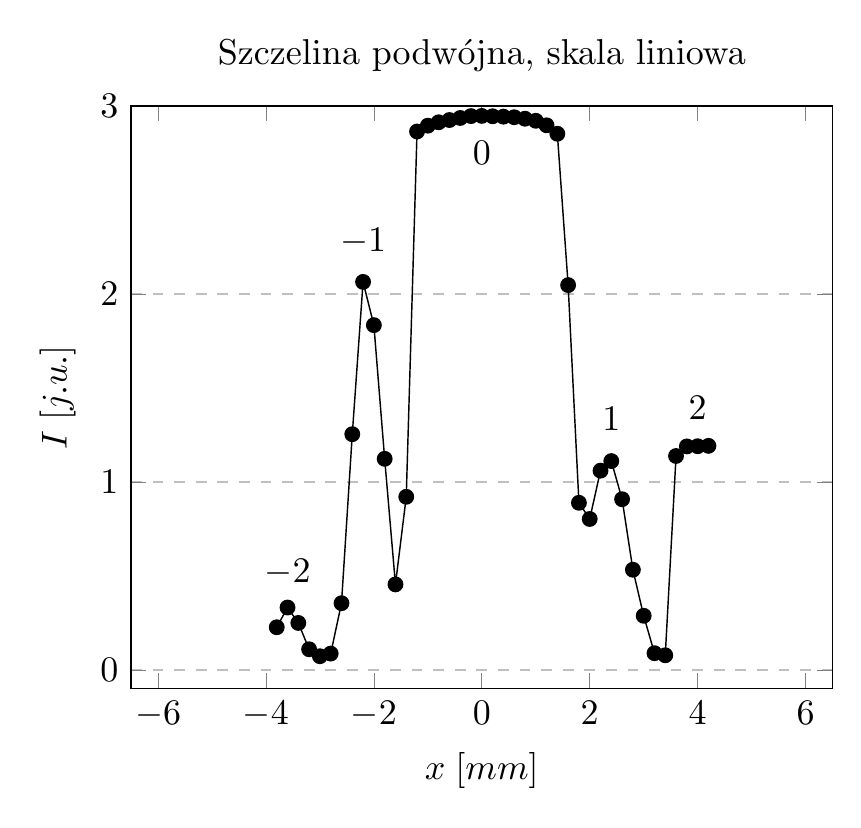
\begin{tikzpicture}[scale=1.3]
\begin{axis}[
title={Szczelina podwójna, skala liniowa},
xlabel={$x\;[mm]$},
ylabel={$I\;[j.u.]$},
xmin=-6.5,xmax=6.5,
ymin=-0.1,ymax=3,
legend pos=north west,
ymajorgrids=true,grid style=dashed
]

\addplot[color=black, mark=*]
coordinates {
(-3.8,0.227)
(-3.6,0.332)
(-3.4,0.250)
(-3.2,0.110)
(-3,0.073)
(-2.8,0.087)
(-2.6,0.355)
(-2.4,1.254)
(-2.2,2.064)
(-2,1.834)
(-1.8,1.123)
(-1.6,0.455)
(-1.4,0.921)
(-1.2,2.864)
(-1,2.895)
(-0.8,2.913)
(-0.6,2.925)
(-0.4,2.936)
(-0.2,2.946)
(0,2.947)
(0.2,2.945)
(0.4,2.943)
(0.6,2.940)
(0.8,2.932)
(1,2.921)
(1.2,2.897)
(1.4,2.852)
(1.6,2.047)
(1.8,0.889)
(2,0.803)
(2.2,1.060)
(2.4,1.111)
(2.6,0.908)
(2.8,0.533)
(3,0.288)
(3.2,0.089)
(3.4,0.078)
(3.6,1.138)
(3.8,1.189)
(4,1.190)
(4.2,1.192)
};
\node[label={270:{$0$}}] at (axis cs: 0,2.947) {};
\node[label={90:{$1$}}] at (axis cs: 2.4,1.140) {};
\node[label={90:{$2$}}] at (axis cs: 4,1.195) {};
\node[label={90:{$-1$}}] at (axis cs: -2.2,2.073) {};
\node[label={90:{$-2$}}] at (axis cs: -3.6,0.315) {};

\end{axis}
\end{tikzpicture}
\end{center}
\begin{center}
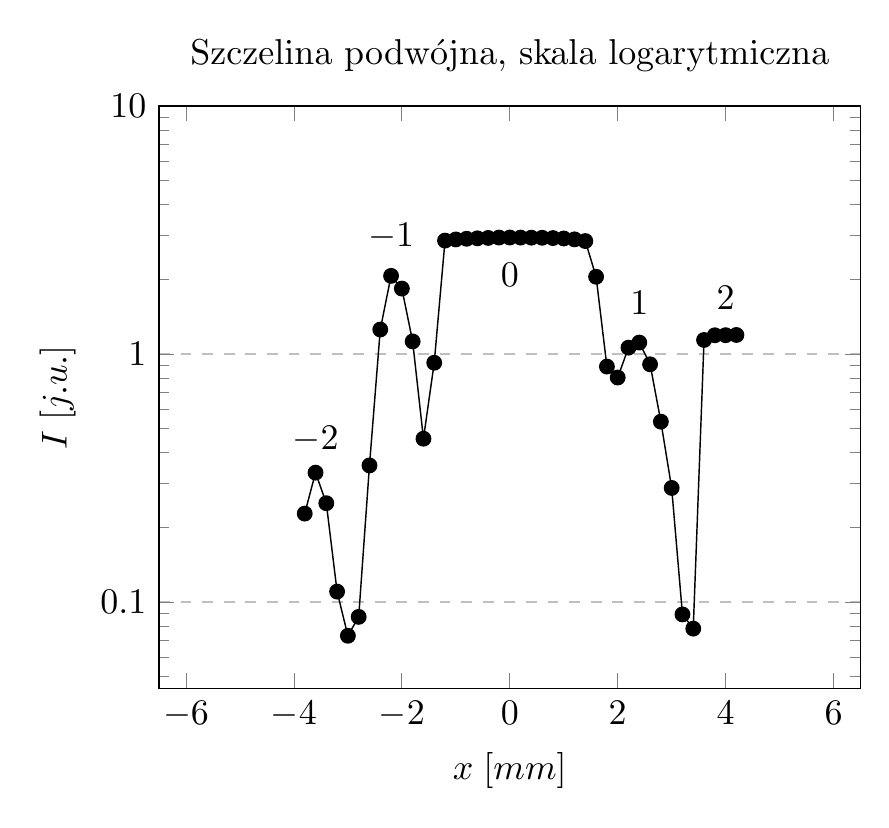
\begin{tikzpicture}[scale=1.3]
\begin{axis}[
title={Szczelina podwójna, skala logarytmiczna},
xlabel={$x\;[mm]$},
ylabel={$I\;[j.u.]$},
xmin=-6.5,xmax=6.5,
ymin=-0.1,ymax=10,
legend pos=north west,
ymajorgrids=true,grid style=dashed,
ymode=log,
log ticks with fixed point,
scaled y ticks=real:1e3
]

\addplot[color=black, mark=*]
coordinates {
(-3.8,0.227)
(-3.6,0.332)
(-3.4,0.250)
(-3.2,0.110)
(-3,0.073)
(-2.8,0.087)
(-2.6,0.355)
(-2.4,1.254)
(-2.2,2.064)
(-2,1.834)
(-1.8,1.123)
(-1.6,0.455)
(-1.4,0.921)
(-1.2,2.864)
(-1,2.895)
(-0.8,2.913)
(-0.6,2.925)
(-0.4,2.936)
(-0.2,2.946)
(0,2.947)
(0.2,2.945)
(0.4,2.943)
(0.6,2.940)
(0.8,2.932)
(1,2.921)
(1.2,2.897)
(1.4,2.852)
(1.6,2.047)
(1.8,0.889)
(2,0.803)
(2.2,1.060)
(2.4,1.111)
(2.6,0.908)
(2.8,0.533)
(3,0.288)
(3.2,0.089)
(3.4,0.078)
(3.6,1.138)
(3.8,1.189)
(4,1.190)
(4.2,1.192)
};
\node[label={270:{$0$}}] at (axis cs: 0,2.947) {};
\node[label={90:{$1$}}] at (axis cs: 2.4,1.140) {};
\node[label={90:{$2$}}] at (axis cs: 4,1.195) {};
\node[label={90:{$-1$}}] at (axis cs: -2.2,2.073) {};
\node[label={90:{$-2$}}] at (axis cs: -3.6,0.315) {};
\end{axis}
\end{tikzpicture}
\end{center}
\subsection{Położenia maksimów}
\begin{figure}[H]
\centering
\includegraphics[width=18cm]{Tab5}
\caption*{\textbf{Tab. 5}: Położenia maksimów natężenia światła}
\end{figure}
\subsection{Wartości średnie i niepewności}
Przy pomocy odczytanych maksimów w Tab. 5 obliczyliśmy wartości średnie współrzędnych $x$ korzystając ze wzoru $x=\frac{x_p-x_l}{2}$. W kolejnym kroku obliczyliśmy wartości szerokości szczeliny $d$ dla każdego maksimum bocznego. W tym celu użyliśmy wzoru: \newline \newline
{\Large $x_{max}=m\frac{\lambda{L}}{d}\;\;\;=>\;\;\;d=m\frac{\lambda{L}}{x_{max}}$} \newline \newline
Dla $1$ maksimum wartości wyniosły: \newline \newline
{\Large $ x=\frac{x_p-x_l}{2}=\frac{2.4\;mm-(-2.2\;mm)}{2}=2.3\;mm \newline
d=m\frac{\lambda{L}}{x_{max}}=1*\frac{650\;nm*755\;mm}{2.3\;mm}=0.214\;mm$} \newline \newline
Drugą wartość obliczyliśmy w analogiczny sposób. 
Następnie obliczyliśmy średnią wartość szerokości szczeliny $\bar{d}=\frac{d_1+d_2}{2}=0.2360\;mm$. By obliczyć niepewność pomiaru szerokości szczeliny $d$ (niepewność typu A) użyliśmy wzoru: \newline \newline
{\Large $u(d)=\sqrt{\frac{\sum_{i=1}^{i=n} (d_i-\bar{d})^2}{n(n-1)}}=\sqrt{\frac{\sum_{i=1}^{i=2} (d_i-\bar{d})^2}{2*1}}=0.022\;mm$}
\subsection{Stosunek natężenia w najbliższym minimum $I_{min}$ do natężenia światła w maksimum $I_0$}
Natężenie światła w maksimum głównym wyniosło $I_{max}=2.947\;j. u.$. Z wykresu odczytaliśmy wartość natężenia światła w pierwszym minimum $I_{min}=0.816\;j. u.$. Stosunek 
$\frac{I_{min}}{I_{max}}$ wynosi: \newline
{\Large $\frac{I_{min}}{I_{max}}=\frac{0.816\;j. u.}{2.947\;j. u.}= 0.277$} \newpage
\section{Wnioski} 
Zmierzona wartość szerokości szczeliny dla pomiarów dla pojedynczej szczeliny wynosi $d=0.2130\;mm$ z niepewnością pomiarową $u(d)=0.0052\;mm$, zaś dla podwójnej szczeliny $d=0.214\;mm$ z niepewnością pomiarową $u(d)=0.022\;mm$. Porównanie niepewności pomiarowych oraz wykresów pozwala stwierdzić, że 
pomiary dla podwójnej szczeliny okazały się o wiele mniej dokładne niż dla pojedynczej. Dla pojedynczej szczeliny względne natężenie doświadczalne dla $1$ i $2$ maksimum bocznego wyniosło odpowiednio $0.05452$,$0.00935$. Względne natężenie teorytyczne to odpowiednio $0.04503$ oraz $0.01621$. Natężenie doświadczalne różni się zatem od teorytycznego odpowiednio o $21\%$ i $42\%$. Dla podwójnej szczeliny stosunek natężenia w najbliższym minimum $I_{min}$ do natężenia światła w maksimum $I_0$ wynosi $\frac{I_{min}}{I_{max}}=0.277$. Wynik jest dosyć odległy od $0$ więc jest on daleki od idealnego.
Wyniki pomiarów pozwalają stwierdzić, że wykonane ćwiczenie jest dobrą metodą pomiaru szerokości szczeliny. Świadczy o tym bardzo mała niepewność pomiarowa $u(d)$. Pomiary natężeń nie okazały się jednak takie dokładne. Jednym z powodów mogą być duże wahania wskazań detektora oraz niedokładność pomiaru odległości szczeliny od ekranu oraz fotodiody od maksimum głównego. Innym powodem mogła być obecność innego, zmiennego źródła światła w pomieszczeniu, w którym wykonywaliśmy doświadczenie.
\end{document}
